\documentclass[11pt]{article}
\usepackage{graphicx}
\usepackage{geometry}
 \geometry{
 a4paper,
 left=20mm,
 right=20mm,
 top=20mm,
 bottom=20mm,
 }
\begin{document}
	\begin{minipage}{0.5\textwidth}
\huge{Aayush Ojha}\\
\normalsize
\emph{Second Year BTech Student} \hfill \\ \emph{Phone No: +91 9793399818}\\
\emph{Computer Science and Engineering} \hfill  \\ \emph{Email : aayushoj@iitk.ac.in}\\
	\end{minipage}
	\begin{minipage}{0.5\textwidth}
\begin{center}
	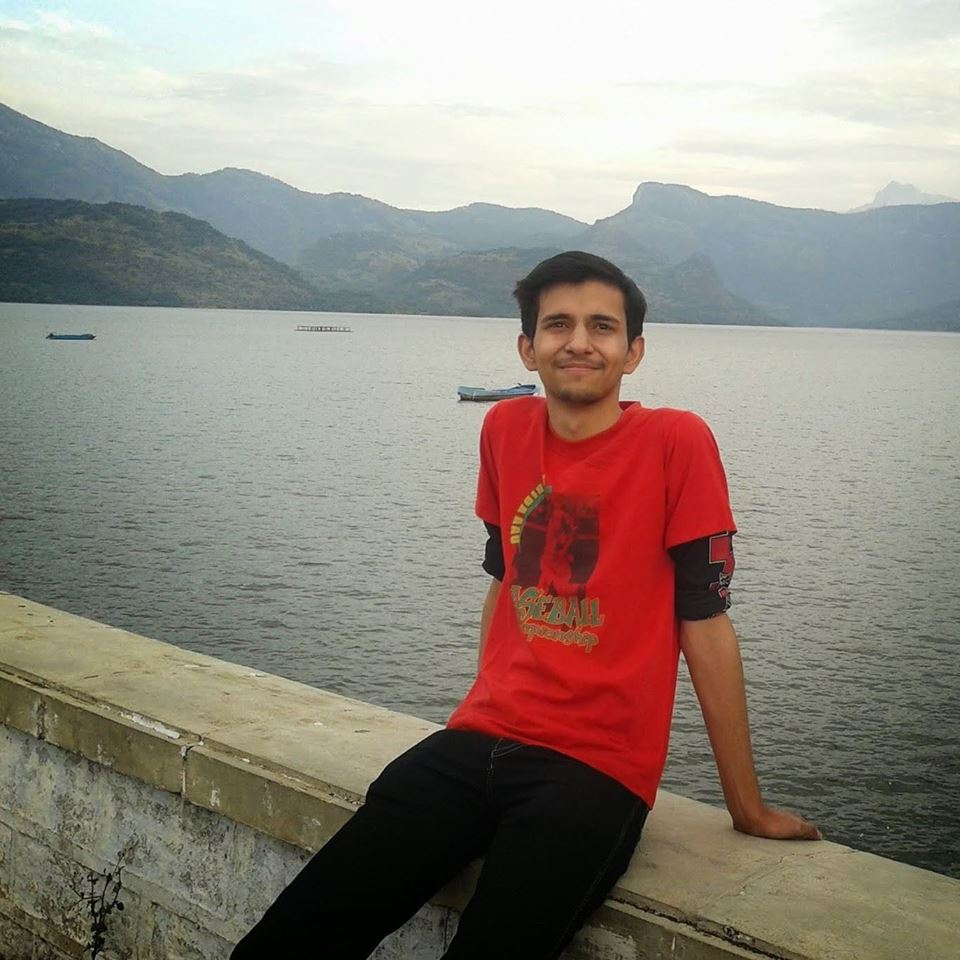
\includegraphics[scale=0.10]{a.eps}\\
\end{center}
	\end{minipage}
	\\
	\\
	\\
\begin{tabular}{|c|c|c|c|}
\hline
\multicolumn{4}{|c|}{Educational Qualifications:}\\[5pt]
\hline
YEAR & DEGREE & INSTITUTION(BOARD) & CGPA/\%\\
\hline
2013-2017 & BTech & Indian Institute of Technology Kanpur & 9.0/10.0\\
\hline
2013 & XII & RLB Mem. Sen. Sec. School & 94.4\\
\hline
2011 & X & R.S.M. Sen. Sec. School & 10.0/10.0\\
\hline
\end{tabular}
\\
\\
\\
\begin{tabular}{ccccccc}
	\multicolumn{7}{c}{PROJECTS:}\\[5pt]
\hline
\end{tabular}
\\
\begin{itemize}
	\item Project under PClub\\
	\item Project under ACA: Developed a programming language to control virtual bots\\
	\item Project under Prof. Amey Karkare: Developing a framework over CodeHunt\\
	\item Course Project TA201A\\
\end{itemize}
\begin{tabular}{ccccccc}
\multicolumn{7}{c}{SCHOLASTIC ACHIEVEMENT:}\\
\hline
\end{tabular}
\\
\begin{itemize}
	\item  Secured 60th rank in ACM-ICPC Asia Amritapuri Regionals ($2014$-$2015$) among $1600$ international teams\\
	\item Secured All India Rank - $138$ in JEE Advanced among more than $500000$ aspirants
\item Secured State Rank -$9$ in UPSEE among more than $140000$ aspirants
\item Secured AIR - $110$ in Kishore Vaigyanik Protsahan Yojana (KVPY) -$2012$
\end{itemize}
\begin{tabular}{|c|c|c|c|c|}
\hline
\multicolumn{5}{|c|}{TRANSCRIPT}\\[5pt]
\hline
COURSE & COURSETYPE & COURSE TITLE & UNITS & GRADES\\
\hline
CS210A & Compulsory & DATA STRUCTURES AND ALGORITHMS & 12 & A*\\
\hline
CS201A & Compulsory & DISCRETE MATHEMATICS & 9 & B\\
\hline
CS251A & Compulsory & COMPUTING LABORATORY-1 & 6 & A*\\
\hline
CS202A & Compulsory & LOGIC IN COMPUTER SCIENCE & 5 & A*\\ 
\hline
TA202A & Compulsory & MANUFACTURING PROCESSES-1 & 6 & D\\
\hline
\end{tabular}
\end{document}
